\chapter{Percolation: k-core \& k-clique percolation}

\resp{Lorenzo Vigorelli}

\section{Percolation}
Percolation describes the effect of progressively removing nodes or edges 
from a network according to specific rules and studying whether a 
macroscopic connected component survives \cite{dedomenico2024dispensa}. 
This process reveals how network structure responds to failures or 
perturbations, and whether the transition from disconnected to connected 
phases is continuous (second order), discontinuous (first order), 
or hybrid. 
Here we focus on local structures, in particular on $k$-clique percolation \cite{derenyi2005clique}.
Regarding the simpler case of percolation in ER networks, consider the procedure explained in the appendix \ref{app:percolation}.

\section{$k$-Clique Percolation}
A \emph{$k$-clique} is a fully connected subgraph of $k$ vertices. 
A \emph{$k$-clique percolation cluster} is built from adjacent cliques 
that share $k-1$ vertices, thus generalizing classical edge percolation. 
In Erdős–Rényi (ER) random graphs, a giant $k$-clique cluster emerges 
when the link probability $p$ exceeds a critical threshold $p_c^{(k)}$, 
which scales as
\begin{equation}
    p_c^{(k)} \simeq \left[(k-1)N^{\tfrac{1}{k-1}}\right]^{-1}.
\end{equation}
For $k=2$, this reduces to the standard ER threshold $p_c = 1/N$.\\
Two natural order parameters can be used:
\begin{align}
    \phi_k &= \frac{N^{*}}{N}, \quad \text{fraction of vertices in the largest cluster,} \\
    \psi_k &= \frac{N_k^{*}}{N_k}, \quad \text{fraction of cliques in the largest cluster.}
\end{align}
Here $N^{*}$ is the number of vertices in the largest $k$-clique cluster, 
$N_k^{*}$ the number of $k$-cliques it contains, and 
\begin{equation}
    N_k \simeq \binom{N}{k} \, p^{k(k-1)/2}
\end{equation}
is the expected total number of $k$-cliques in the network.\\
At the percolation threshold, the scaling of the largest $k$-clique cluster 
with system size $N$ follows \cite{derenyi2005clique}:
\begin{equation}
N_c \sim
\begin{cases}
    N^{-k/6}, & k \leq 3, \\
    N^{\,1 - \tfrac{k}{2}}, & k \geq 3.
\end{cases}
\end{equation}


\section{Simulations}

\begin{figure*}[h!]
    \centering
    \setlength{\tabcolsep}{2pt}
    \begin{minipage}[t]{0.48\textwidth}
        \centering
        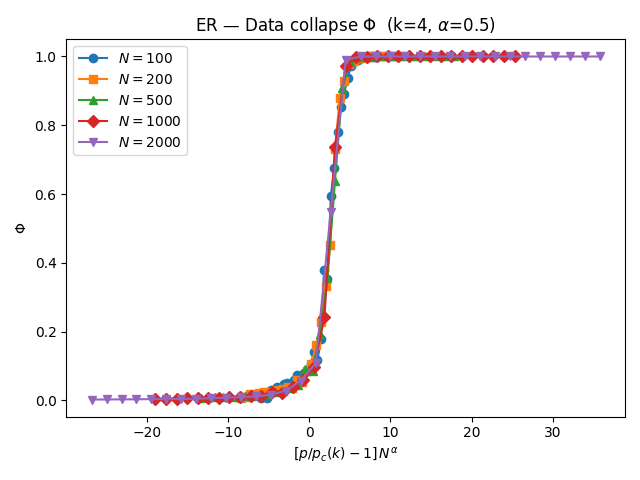
\includegraphics[width=\textwidth]{images/IMAGES TASK2/ER_collapse_phi_k4_alpha0.5.png}
        \subcaption{Scaling collapse with $\alpha=0.45$.}
        \label{fig:collapse_alpha045}
    \end{minipage}
    \hfill
    \begin{minipage}[t]{0.48\textwidth}
        \centering
        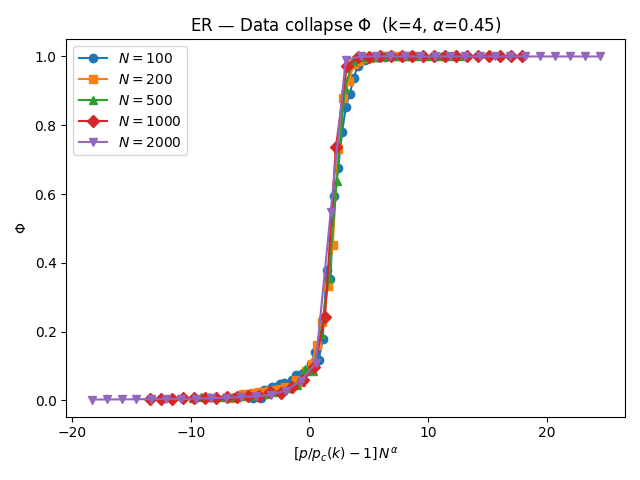
\includegraphics[width=\textwidth]{images/IMAGES TASK2/ER_collapse_phi_k4_alpha0.45.png}
        \subcaption{Scaling collapse with $\alpha=0.50$.}
        \label{fig:collapse_alpha050}
    \end{minipage}
    \caption{Comparison of scaling collapses for $k=4$ using different critical exponents $\alpha$.}
    \label{fig:collapse_k4}
\end{figure*}

\begin{itemize}
\item Collapse when rescaled accordingly with $\alpha=0.45$:  
The scaling collapse in Fig.~\ref{fig:collapse_alpha045} shows an almost universal curve across system sizes $N$.  
However, finite-size effects are still visible, suggesting that $\alpha=0.45$ is not the optimal critical exponent.

\item Collapse where rescaled accordingly with $\alpha=0.50$:  
When using $\alpha=0.50$ (Fig.~\ref{fig:collapse_alpha050}), the collapse is significantly better, with nearly perfect overlap of curves from different $N$.  
This indicates that $\alpha=0.50$ captures the correct finite-size scaling of the order parameter.
\end{itemize}
The contrast between the two panels in Fig.~\ref{fig:collapse_k4} highlights the importance of correctly identifying the critical exponent.  
Notice that the correct $\alpha$ depends on the clique size $k$.
\begin{figure*}[h!]
    \centering
    \setlength{\tabcolsep}{2pt}
    \begin{minipage}[t]{0.48\textwidth}
        \centering
        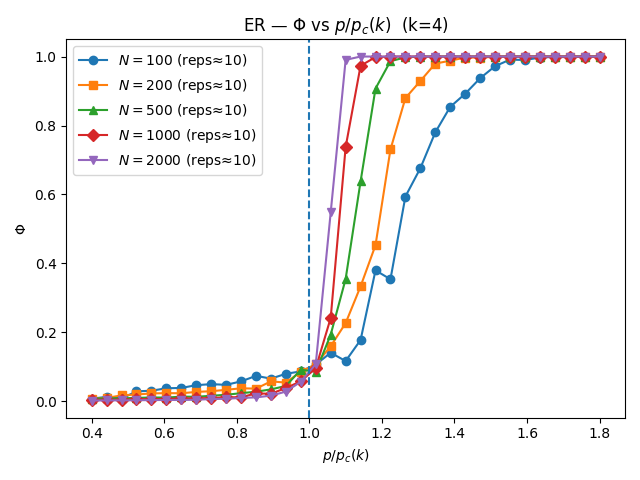
\includegraphics[width=\textwidth]{images/IMAGES TASK2/ER_phi_k4.png}
        \subcaption{Order parameter $\phi_k$ for $k=4$.}
        \label{fig:phi_k4}
    \end{minipage}
    \hfill
    \begin{minipage}[t]{0.48\textwidth}
        \centering
        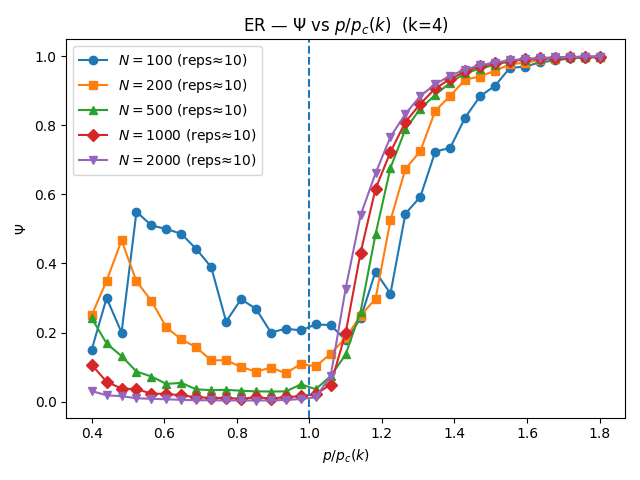
\includegraphics[width=\textwidth]{images/IMAGES TASK2/ER_psi_k4.png}
        \subcaption{Order parameter $\psi$ for $k=4$.}
        \label{fig:psi_k4}
    \end{minipage}
    \caption{Order parameters for $k=4$: relative number of cliques (left) and fraction of vertices (right).}
    \label{fig:orderparam_k4}
\end{figure*}\\
Considering the case $k=4$ (Fig.~\ref{fig:orderparam_k4}):
\begin{itemize}
\item $\psi_k$:  
The relative number of $k$-cliques in the largest cluster increases smoothly with $p$ (Fig.~\ref{fig:psi_k4}).  
This continuous trend suggests a second-order–like transition in clique space, converging to a step function in the thermodynamic limit.
Simulations confirm that curves for different $N$ collapse when rescaled, consistent with theoretical expectations.

\item $\phi$:  
In contrast, the fraction of vertices in the largest $k$-clique cluster (Fig.~\ref{fig:phi_k4}) exhibits a much sharper jump near criticality.  
This nearly discontinuous behavior resembles a first-order transition, even though in the limit $N \to \infty$ it should converge to a function, which is $0$ for $p \leq p_c^{(k)}$ and grows continuously to $1$ for $p > p_c^{(k)}$.

\end{itemize}\\
In summary, for $k=4$ the choice of order parameter is crucial:  
$\psi_k$ suggests continuous growth, while $\phi$ reveals a sharp structural jump.  
This duality illustrates the coexistence of second-order-like behavior in vertex space and first-order-like behavior in clique space.

\begin{figure*}[h!]
    \centering
    \setlength{\tabcolsep}{2pt}
    \begin{minipage}[t]{0.48\textwidth}
        \centering
        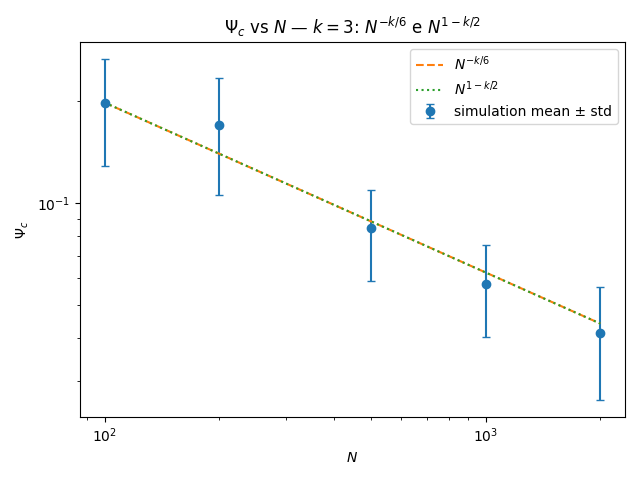
\includegraphics[width=\textwidth]{images/IMAGES TASK2/ER_psic_vsN_k3.png}
        \subcaption{Scaling of $\psi_c$ with $N$ for $k=3$.}
        \label{fig:psic_k3}
    \end{minipage}
    \hfill
    \begin{minipage}[t]{0.48\textwidth}
        \centering
        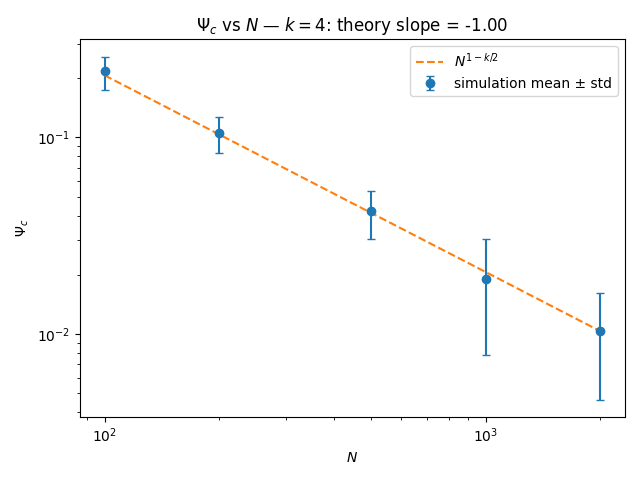
\includegraphics[width=\textwidth]{images/IMAGES TASK2/ER_psic_vsN_k4.png}
        \subcaption{Scaling of $\psi_c$ with $N$ for $k=4$.}
        \label{fig:psic_k4}
    \end{minipage}
    \caption{Scaling of the critical order parameter $\psi_c$ with system size $N$ for $k=3$ and $k=4$.}
    \label{fig:psic_scaling}
\end{figure*}

\begin{itemize}
\item Critical $\psi_c$ vs $N$, $k=3$:  
The scaling in Fig.~\ref{fig:psic_k3} follows the theoretical prediction $\psi_c \sim N^{-2/3}$, showing that the relative size of the giant 3-clique cluster decreases with $N$.  
This implies that, although a giant 3-clique cluster exists for finite networks, its relative weight vanishes in the thermodynamic limit.

\item Critical $\psi_c$ vs $N$, $k=4$:  
For $k=4$, Fig.~\ref{fig:psic_k4} shows an even steeper decrease with $N$, consistent with $\psi_c \sim N^{-1}$.  
This indicates that the giant 4-clique cluster becomes negligible even faster, vanishing completely as $N \to \infty$.  
\end{itemize}\\
The comparison in Fig.~\ref{fig:psic_scaling} highlights the change in scaling:  
for $k=3$, the giant clique cluster shrinks as $N^{-2/3}$, while for $k=4$ it decays more sharply as $N^{-1}$.  
In both cases the relative size tends to zero in the thermodynamic limit, but the suppression is stronger for higher-order cliques. Other analysis in appendix \ref{app:percolation}\\
It would be also particularly interesting to extend this analysis to scale-free networks, exploring how different percolation modes (node/edge, random failures or targeted attacks) affect the nature of the transition. 


\newpage